
\documentclass[../open-optimization/open-optimization.tex]{subfiles}

%%%%%%%%%
\begin{document}
%%%%%%%%%

\titlepic{
	\begin{center}
	\begin{tabular}{ccccc}
	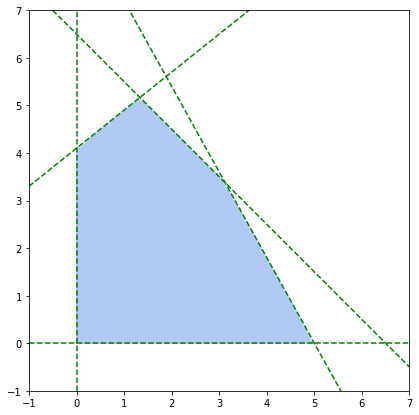
\includegraphics[scale = 0.3]{LP-feasible-region}  & \quad & 
	 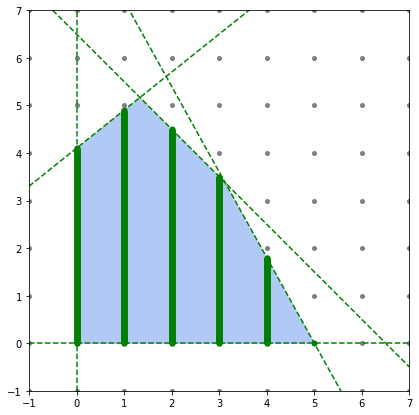
\includegraphics[scale = 0.3]{MIP-feasible-region} & \quad &
	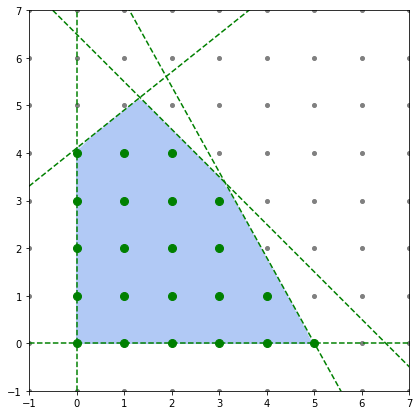
\includegraphics[scale = 0.3]{IP-feasible-region}%% \\
	%% LP && MIP && IP\\
	%% \\
	%% $Ax \leq b$ & &$Ax \leq b$ && $Ax \leq b$\\
	%% & &$x_1 \in \Z$ & &$x_1, x_2 \in \Z$
	\end{tabular}
	\end{center}\nopagebreak
        \begin{center}
          
\includegraphics[width=\linewidth]{../../../open-optimization-common/logos/logo-open-optimization-oer-wide}
        \end{center}
}
\maketitle

%%% Copyright page
\thispagestyle{empty}
%%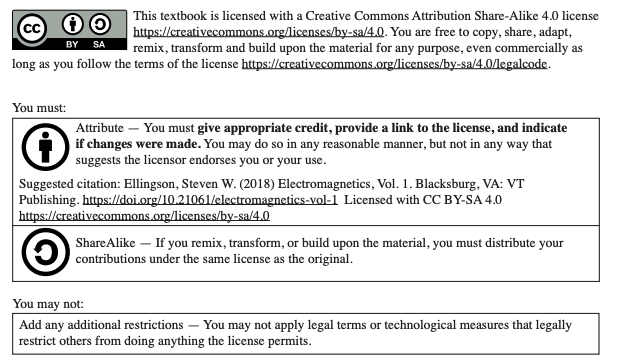
\includegraphics[scale = 0.65]{creative-commons-statement}

\begin{tabular}{p{.3\linewidth}@{\qquad}p{.55\linewidth}}
  \begin{minipage}[c]{\linewidth}
    \centering\Huge\ccCopy
  \end{minipage}
  & \begin{minipage}[c]{\linewidth}
    Copyright 2019 by the contributors listed on the title page.
  \end{minipage}
  \\\\[2ex]
  \begin{minipage}[c]{\linewidth}
    \doclicenseImage[imagewidth=\linewidth]%
  \end{minipage}
  & \begin{minipage}[c]{\linewidth}%
    \doclicenseLongText\par\vspace{-1ex}
    \raggedleft
    \url{https://creativecommons.org/}
  \end{minipage}
  \\\\[2ex]
  \begin{minipage}[c]{\linewidth}
    \centering\Huge\ccShareAlike 
  \end{minipage}
  & \begin{minipage}[c]{\linewidth}
    This license allows everyone to remix, tweak, and build upon this work even for
    commercial purposes\dots
  \end{minipage}
  \\\\[2ex]
  \begin{minipage}[c]{\linewidth}
    \centering\Huge\ccAttribution
  \end{minipage}
  & \begin{minipage}[c]{\linewidth}
    \dots as long as they credit the copyright holders and license their new
    creations under the identical terms.
  \end{minipage}
  \\\\[2ex]
    \begin{minipage}[c]{\linewidth}
    \includegraphics[width=\linewidth]{../../../open-optimization-common/logos/Global_Open_Educational_Resources_Logo.svg}\footnotemark
  \end{minipage}
  & \begin{minipage}[c]{\linewidth}
    This work aligns with the mission of UNESCO Open Educational
    Resources.\par\vspace{1ex}
    \raggedleft
    \url{https://en.unesco.org/themes/building-knowledge-societies/oer}
  \end{minipage}
  \\\\[2ex]
  \begin{minipage}[c]{\linewidth}
    \centering\LARGE\LaTeX
  \end{minipage}
  & \begin{minipage}[c]{\linewidth}
    The source code of this book is available.\par\vspace{1ex}
    \raggedleft
    \url{https://github.com/open-optimization/}
  \end{minipage}
\end{tabular}

\begin{center}
\end{center}
\footnotetext{\url{https://en.wikipedia.org/wiki/Open_educational_resources\#/media/File:Global_Open_Educational_Resources_Logo.svg}}

\newpage

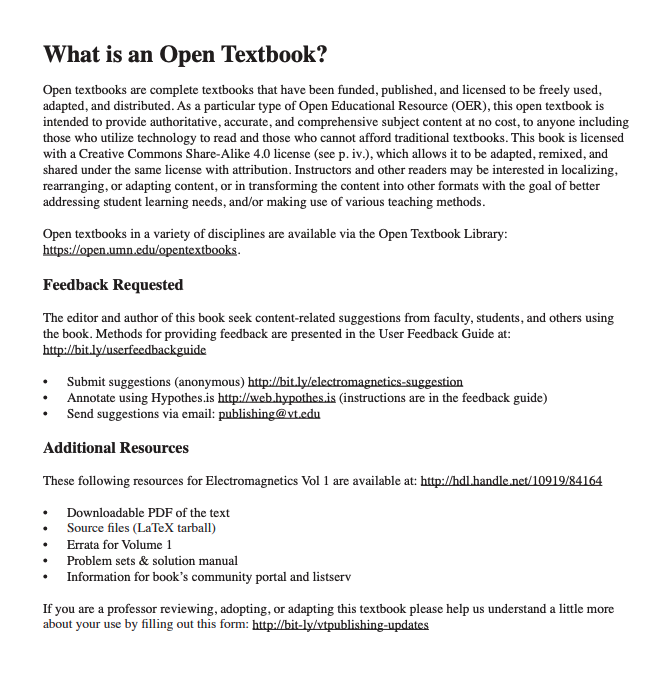
\includegraphics[scale = 0.65]{what-is-open-textbook}\footnotemark
\footnotetext{Take from open-source electromagnetics book}

\newpage

\section*{Preface}
\hypertarget{moved-here-from-open-optimization-or-bookcontentintro-mathprog-oropen-optimization-sectionsfront-matter.tex}{%
\subsection{Moved here from
open-optimization-or-book/content/intro-mathprog-or/open-optimization-sections/front-matter.tex}\label{moved-here-from-open-optimization-or-bookcontentintro-mathprog-oropen-optimization-sectionsfront-matter.tex}}

Welcome to the Open Optimization - an ecosystem for open-source
materials for teaching optimization and operations research. This
ecosystem is being formed to host open-source lecture notes, lecture
slides, examples, code, figures, and textbooks on material and courses
related to optimization. All material will be licensed under Creative
Commons Attribution-ShareAlike 4.0 International (CC BY-SA 4.0) that
permits free reuse and alteration of the material provided the proper
attribution is given. All material posted will be not just open-source,
but open-source code as well - including LaTeX, tikz, and other means of
generating content. This allows those interested in reusing material an
easy way to change and adapt the material as needed.

Your contributions to this endeavor are greatly valued and appreciated.
You are being contacted directly due to the excellent material that you
have on your website. We hope you will help with this project and also
use it as a resource for future courses, lectures, and presentations.

Content posted here may be adapted into freely available open-source
textbooks published through ???. All contributors to this repository
will be acknowledged in any publication resulting from this material.
Please see ???? as an example.

Goals:

\begin{enumerate}
\def\labelenumi{\arabic{enumi}.}
\item
  Create freely available content to make easier teaching, designing
  courses, writing presentations, and finding reusable content.
\item
  Create free textbooks for courses on optimization and operations
  research that are:

  \begin{itemize}
  \tightlist
  \item
    Modern (up to date with current techniques and approaches)
  \item
    Flexible (easy to adapt to the user's choice of presentation of
    material)
  \item
    Connected to code examples (get students up and running faster)
  \end{itemize}
\item
  Community collaboration on content authoring and revisions
\item
  Collect figures and images with source code for quality
  reproducibility
\item
  Host instructive code for optimization
\end{enumerate}

%\hypertarget{preface-material-adapted-from-the-open-electromagnetics-project---to-edit}{%
%\subsection{PREFACE material adapted from The Open Electromagnetics
%Project - to
%edit}\label{preface-material-adapted-from-the-open-electromagnetics-project---to-edit}}
%
%While a number of very fine traditional textbooks are available on this
%topic, we feel that it has become unreasonable to insist that students
%pay hundreds of dollars per book when effective alternatives can be
%provided using modern media at little or no cost to the student. This
%project is equally motivated by the desire for the freedom to adopt,
%modify, and improve educational resources. This work is distributed
%under a Creative Commons BY\textasciitilde{}SA license which allows --
%and we hope encourages -- others to adopt, modify, improve, and expand
%the scope of our work.
%
%Finally, we acknowledge all those who have contributed their art to
%Wikimedia Commons (https://commons.wikimedia.org/) under open licenses,
%allowing their work to appear as figures in this book. These
%contributors are acknowledged in figures and in the ``Image Credits''
%section at the end of each chapter. Thanks to each of you for your
%selfless effort.

%\hypertarget{why-cite-wikipedia-pages-as-additional-reading}{%
%\subsubsection{Why cite Wikipedia pages as additional
%reading?}\label{why-cite-wikipedia-pages-as-additional-reading}}
%
%Many modules cite Wikipedia entries as sources of additional
%information. Wikipedia represents both the best and worst that the
%Internet has to offer. Most educators would agree that citing Wikipedia
%pages as primary sources is a bad idea, since quality is variable and
%content is subject to change over time. On the other hand, many
%Wikipedia pages are excellent, and serve as useful sources of relevant
%information that is not strictly within the scope of the curriculum.
%Furthermore, students benefit from seeing the same material presented
%differently, in a broader context, and with the additional references
%available as links from Wikipedia pages. We trust instructors and
%students to realize the potential pitfalls of this type of resource and
%to be alert for problems.


%%%%%%%%%
\end{document}
%%%%%%%%%
%%% Local Variables:
%%% mode: latex
%%% TeX-master: "../open-optimization/open-optimization"
%%% End:
